\subsection{Glyph: \glyph{Equivalence}}
\label{sec:equivalence}
%The glyph \glyph{equivalence} is used to denote that all the \glyph{EPNs} linked as input are necessary to produce the output.  
\add{The \glyph{equivalence operator} provides a mechanism to sub-class EPNs. For example, this operator allows specifying that macromolecules or nucleic acid features X\textsubscript{1}, X\textsubscript{2}, and X\textsubscript{3} are subclasses of X. This avoids the need for processes that apply to all subtypes of X to be duplicated and simplifies cases where combinatorial explosions of the number of EPNs or PNs may arise. Caution should be used with this glyph as there is the possibility that ambiguity may be introduced into a SBGN map. Examples of the correct usage of this glyph are provided in Appendix~\ref{ex_eq} together with examples of misuse along with a proposed set of guidelines for the use of this \glyph{equivalence operator}.}

\luna{this section is written very differently from the others. text like "until now" may have no purpose years later when people read this. TEXT BEFORE 032819: 
Until now, the SBGN Process Description language has not provided mechanisms to sub-class EPNs.
There was no specific means of specifying that macromolecules or nucleic acid features \corr{X1}{X\textsubscript{1}}, \corr{X2}{X\textsubscript{2}}, and \corr{X3}{X\textsubscript{3}} are subclasses of X.
Therefore, any process that applies to all the subtypes of X had to be triplicated.
That situation could easily generate combinatorial explosions of the number of EPNs or PNs.

To enable the representation of EPNs together with corresponding sub-classes of this EPNs, we introduce the equivalence operator glyph.
Please note that this glyph can potentially introduce ambiguity.
Examples of the correct use of the glyph are provided in Appendix~\ref{ex_eq} together with examples of misuse and with the proposed set of rules suggested as guideline for the use of the \glyph{equivalence operator}.}

\begin{glyphDescription}

\glyphSboTerm
SBO:0000392 ! equivalence\corr{ (is a)}{}

\corr{
\glyphOrigin More than one \glyph{EPN} (section~\ref{sec:EPNs}).
}{
\glyphIncoming Two or more \glyph{logic arcs} (\sect{logicArc}).
}

\corr{
\glyphTarget  One logic arc (section~\ref{sec:logicArc}).
}{
\glyphOutgoing
One \glyph{logic arc} (\sect{logicArc}).
}

\glyphContainer
An \glyph{equivalence} operator is represented by a circular shape containing the symbol ``$\Xi$'' (letter ``xi'' of the Greek alphabet\add{)}.
The choice of the symbol is motivated by its use in mathematics for describing relationships as ``equivalent to'' or ``identical to''.
% \rougny{In my opinion, this shows that the equivalence operator should not be a logical operator (and even not an operator at all), because it represents a relationship (it does not produce anything, on the contrary to operators)}
The shape is linked to two ports, that are small arcs attached to the centres of opposite sides of the shape, as shown in \fig{equivalenceOperator}.
\corr{The incoming \glyph{logic arcs} (\sect{logicArc}) are linked to the extremity of the leftmost or uppermost port, while the outgoing \glyph{logic arc} (\sect{logicArc}) is linked to the extremity of the rightmost or bottommost port.}{}

\glyphLabel
\corr{An \glyph{equivalence} operator is not identified by any label}{None}.

\glyphAux
\corr{An \glyph{equivalence} operator does not carry any auxiliary items}{None}.

\end{glyphDescription}

\begin{figure}[H]
  \centering
  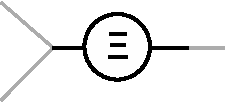
\includegraphics{images/equivalence}
  \caption{The \PD glyph for \glyph{equivalence operator}. Only two inputs are represented, but more would be allowed.}
  \label{fig:equivalenceOperator}
\end{figure}

\add{
The example of \fig{D1_1} presents the binding of different forms of TNF$\alpha$ to two receptors, TNFR1 and TNFR2.
Only membrane TNF$\alpha$ (mTNF$\alpha$) can bind to TNFR2, while both membrane TNF$\alpha$ and soluble TNF$\alpha$ (sTNF$\alpha$) can bind to TNFR1.
Binding of both forms to TNFR1 can conveniently be represented using a generic form of TNF$\alpha$, that is built using an \glyph{equivalence operator}.
}

\begin{figure}
\begin{center}
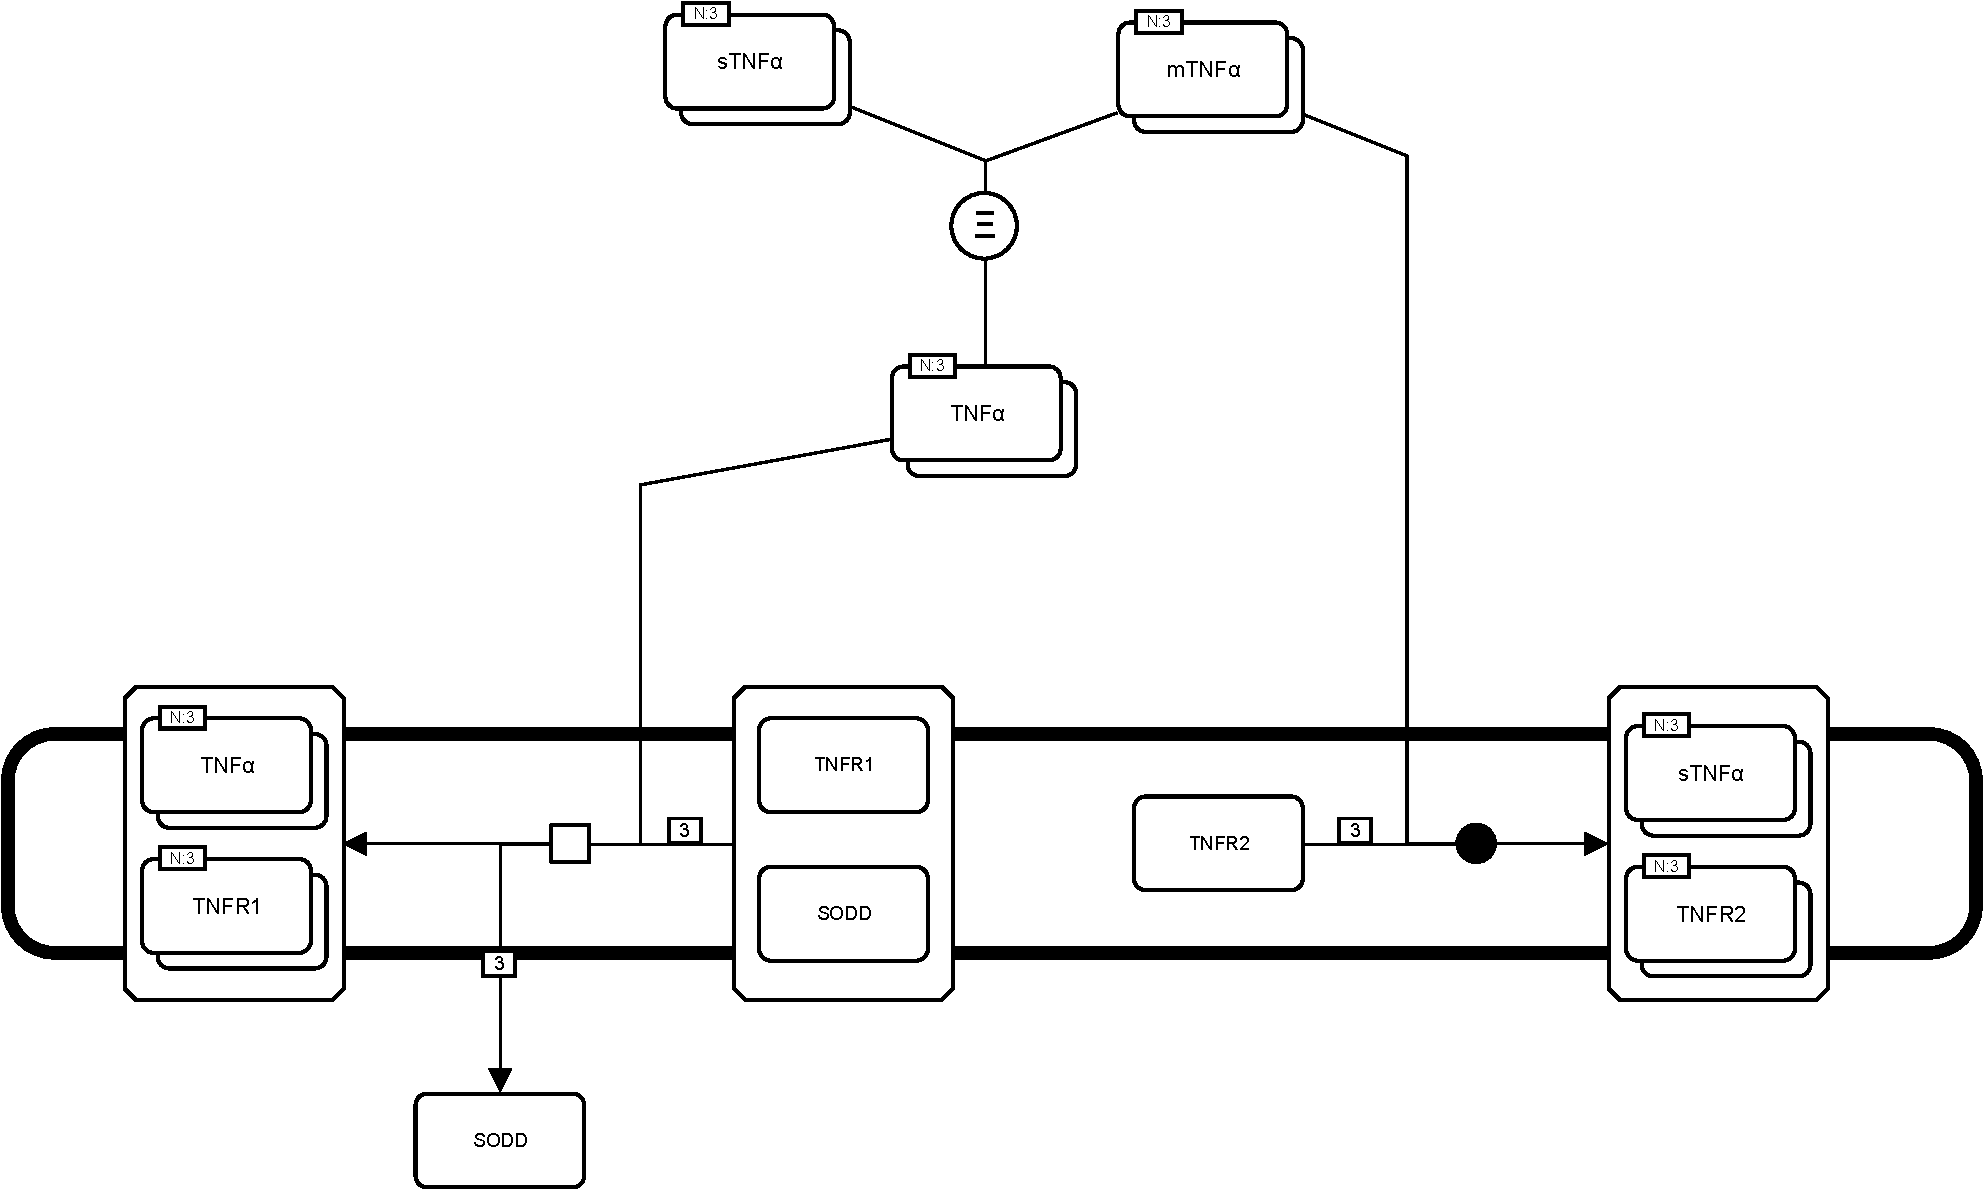
\includegraphics[scale=0.45]{examples/D1_1}
\end{center}
\caption{Binding of diverse forms of TNF$\alpha$ to TNF receptors.}
\label{fig:D1_1}
\end{figure}



% \begin{center}
% \scalebox{0.5}{\includegraphics{images/stimulation-example1}}
% \end{center}
